\title{\textbf{Compressed MHA: Joint Truncated SVD for Multi-Architecture Attention Compression}}

\author{Anonymous authors}


\section{Introduction}

\subsection{Motivation}

The four attention projection matrices $W_Q, W_K, W_V, W_O \in \mathbb{R}^{d \times d}$ 
together contain $4 d^2$ parameters per layer -- for $d = 768$, that's **2.36M 
parameters per layer**, dominating the attention block. Across 12 layers of 
RoBERTa, this is \textbf{28.3M parameters} just in projections.

Low-rank factorization reduces this cost. For a matrix $W \in \mathbb{R}^{d \times d}$, 
SVD replaces it with $U_r V_r$ where $U_r \in \mathbb{R}^{d \times r}$, 
$V_r \in \mathbb{R}^{r \times d}$, and $r \ll d$. Parameter count drops from 
$d^2$ to $2 r d$.

\textbf{Standard SVD compression} treats each projection independently:

\[
W_Q \to U_{Q,r} V_{Q,r}, \quad W_K \to U_{K,r} V_{K,r}, \quad W_V \to U_{V,r} V_{V,r}, \quad W_O \to U_{O,r} V_{O,r}
\]

This costs $4 \cdot 2 r d = 8 r d$ parameters.

\textbf{Key observation.} In pretrained transformers, the Q, K, V projections of a 
head are \textbf{highly correlated} -- they share a common input basis. This suggests 
that a \textbf{shared} input-space basis $V_{QKV}$ may capture the structure of all 
three with minimal loss.

\subsection{Problem Statement}

Given a pretrained transformer $\mathcal{M}$ with hidden dimension $d$ and 
head dimension $d_h$, we seek compressed projections 
$\{W_Q, W_K, W_V, W_O\}$ such that:

\[
\text{Cost}(\mathcal{A}') \ll 4 d^2, \qquad
\mathcal{A}' \approx \mathcal{A}
\]

subject to:

\begin{enumerate}
\item \textbf{Parameter reduction:} Compressed projection count $< 4 d^2$.
\item \textbf{Accuracy preservation:} Near-baseline on SST-2.
\item \textbf{Multi-architecture:} Support flat, nested, causal, and GQA models.
\item \textbf{Recovery capacity:} LoRA adapters for fine-tuning.
\item \textbf{Correctness:} Handle nested encoders without double projection.

\end{enumerate}
\subsection{Our Approach: Joint QKV SVD}

We stack the Q, K, V projections:

\[
W_{QKV} = \begin{pmatrix} W_Q \\ W_K \\ W_V \end{pmatrix} \in \mathbb{R}^{(d + 2 d_{kv}) \times d}
\]

where $d_{kv} = H_{kv} \cdot d_h$ for grouped-query attention.

We then compute a single SVD:

\[
W_{QKV} = U_{QKV} \Sigma_{QKV} V_{QKV}^\top
\]

and truncate to rank $r$:

\[
W_{QKV} \approx U_{QKV, r} \Sigma_{QKV, r}^{1/2} \cdot \Sigma_{QKV, r}^{1/2} V_{QKV, r}^\top
\]

\textbf{Advantages:}

\begin{enumerate}
\item \textbf{Shared basis:} $V_{QKV, r}$ is a single input basis for Q, K, V.
\item \textbf{Smaller parameter count:} $r(d + 2d_{kv}) + r \cdot d = 2rd + 2r d_{kv}$ vs
  independent $6rd$.
\item \textbf{Correlation exploitation:} SVD automatically captures the shared
  structure.

\end{enumerate}
We apply separate SVD to the output projection $W_O \in \mathbb{R}^{d \times d_h H}$:

\[
W_O \approx U_{O, r} \Sigma_{O, r}^{1/2} \cdot \Sigma_{O, r}^{1/2} V_{O, r}^\top
\]

\subsection{Contributions}

\begin{itemize}
\item \textbf{Joint QKV SVD.} We propose stacking Q, K, V and factorizing them with a
  single SVD, sharing the input basis across all three projections.
\item \textbf{Multi-architecture support.} The implementation handles flat (DistilBERT),
  nested (RoBERTa), Conv1D (GPT-2), and GQA+RoPE (Qwen) models.
\item \textbf{Correct nested-encoder detection.} We check for \texttt{out\_lin} / \texttt{c\_proj} /
  \texttt{o\_proj} \textbf{before} declaring a model nested, fixing a subtle double-
  projection bug that caused 50.92\% collapse in earlier implementations.
\item \textbf{Safe failure handling.} Weight extraction failures trigger warnings, not
  exceptions, allowing graceful degradation.
\item \textbf{LoRA recovery on both branches.} Both the QKV and output branches have
  independent LoRA adapters.
\item \textbf{Honest parameter accounting.} We report exact parameter reductions.

\end{itemize}
\subsection{Paper Organization}

Section 2 reviews related work. Section 3 provides background on SVD, LoRA, 
and attention. Section 4 presents Compressed MHA. Section 5 describes 
integration. Section 6 details the setup. Section 7 reports results. Section 8 
analyzes trade-offs. Section 9 discusses practical guidance. Section 10 lists 
limitations. Section 11 concludes.



\subsection{Notation}

\begin{lstlisting}

---
\end{lstlisting}

\section{Related Work}

\subsection{Low-Rank Factorization}

\textbf{Classical SVD.} Eckart-Young theorem gives the optimal rank-$r$ 
approximation in Frobenius norm. We apply this to attention projections.

\textbf{Linformer} (Wang et al., 2020) projects K, V to a fixed sequence dimension 
using learned matrices E, F. This is a different axis of compression 
(sequence, not feature).

\textbf{ALBERT} (Lan et al., 2020) shares parameters across layers, exploiting 
cross-layer redundancy. Our method exploits \textbf{intra-layer} Q/K/V correlation.

\textbf{Nystr mformer} (Xiong et al., 2021) uses Nystr m landmarks for attention 
approximation, not projection compression.

\subsection{Attention Compression}

\textbf{Multi-Query Attention (MQA)} (Shazeer, 2019) shares K, V across all query 
heads, reducing KV parameters by $H/H_{kv}$. \textbf{Grouped-Query Attention (GQA)} 
(Ainslie et al., 2023) is a generalization.

\textbf{Multi-Head Latent Attention (MLA)} (DeepSeek-V2, 2024) projects KV to a 
low-rank latent. This is a \textbf{sequence-level} projection.

\textbf{Our distinction.} We compress the \textbf{weight matrices} directly, sharing 
the input basis across Q, K, V via joint SVD. This is orthogonal to 
sequence-level compression methods.

\subsection{Structured Pruning}

\textbf{Structured pruning} removes entire channels. \textbf{SVD-based methods} 
(like ours) factorize instead.

\textbf{Sliding window + SVD} hybrids exist (SVD-LLM, etc.), but we do not 
combine these.

\subsection{Parameter-Efficient Fine-Tuning}

\textbf{LoRA} (Hu et al., 2021) freezes base weights and trains low-rank adapters. 
\textbf{AdaLoRA} (Zhang et al., 2023) allocates rank adaptively. \textbf{DoRA} (Liu 
et al., 2024) decomposes magnitude and direction.

\textbf{Our use.} We freeze SVD factors and apply LoRA on top, allowing 
recovery fine-tuning without undoing the compression.

\subsection{Position of Our Work}

\begin{table}[H]
\centering
\small
\begin{tabular}{llll}
\toprule
\textbf{Method} & \textbf{Axis} & \textbf{Joint?} & \textbf{Params reduction} \\
\midrule
Linformer & Sequence & No & No (adds params) \\
MQA/GQA & KV heads & No & Yes \\
MLA & Sequence latent & No & Yes \\
\textbf{Compressed MHA} & \textbf{Feature (weights)} & \textbf{Yes (QKV)} & \textbf{Yes} \\
\bottomrule
\end{tabular}
\end{table}

\textbf{Key distinction.} Compressed MHA is the first to jointly factorize Q, K, V 
with a shared input basis, exploiting intra-layer correlation. This yields 
smaller compressed matrices than independent SVD.



\subsection{Comparison Table}

\begin{lstlisting}

---
\end{lstlisting}

\section{Background}

\subsection{Multi-Head Self-Attention}

For input $X \in \mathbb{R}^{B \times L \times d}$:

\[
Q = X W_Q, \quad K = X W_K, \quad V = X W_V
\]

where $W_Q \in \mathbb{R}^{d \times H \cdot d_h}$, $W_K, W_V \in \mathbb{R}^{d \times H_{kv} \cdot d_h}$.

The output projection:

\[
\text{Out} = \text{Attn}(Q, K, V) W_O
\]

where $W_O \in \mathbb{R}^{H \cdot d_h \times d}$.

\subsection{Multi-Head Attention Parameters}

\begin{table}[H]
\centering
\small
\begin{tabular}{lll}
\toprule
\textbf{Projection} & \textbf{Shape} & \textbf{Params} \\
\midrule
$W_Q$ & $d \times H d_h$ & $d H d_h$ \\
$W_K$ & $d \times H_{kv} d_h$ & $d H_{kv} d_h$ \\
$W_V$ & $d \times H_{kv} d_h$ & $d H_{kv} d_h$ \\
$W_O$ & $H d_h \times d$ & $d H d_h$ \\
\bottomrule
\end{tabular}
\end{table}

For standard MHA ($H = H_{kv}$):
\[
\text{Total} = 4 d^2
\]

\subsection{Singular Value Decomposition}

For $W \in \mathbb{R}^{m \times n}$:

\[
W = U \Sigma V^\top
\]

where $U \in \mathbb{R}^{m \times m}$, $\Sigma \in \mathbb{R}^{m \times n}$ diagonal, 
$V \in \mathbb{R}^{n \times n}$ orthogonal.

\textbf{Truncated SVD.} Rank-$r$ approximation:

\[
W_r = U_{:, :r} \Sigma_{:r, :r} V_{:r, :}^\top
\]

\textbf{Error.} $\|W - W_r\|_F = \sqrt{\sum_{i > r} \sigma_i^2}$.

\subsection{Symmetric Factorization}

For numerical stability, distribute $\Sigma^{1/2}$:

\[
W_r = \underbrace{U_{:, :r} \Sigma_{:r, :r}^{1/2}}_{U_r'} \underbrace{\Sigma_{:r, :r}^{1/2} V_{:r, :}^\top}_{V_r'}
\]

Both factors have balanced magnitude.

\subsection{Joint QKV Stacking}

Instead of separate SVD per projection, we stack:

\[
W_{QKV} = \begin{pmatrix} W_Q \\ W_K \\ W_V \end{pmatrix} \in \mathbb{R}^{(H d_h + 2 H_{kv} d_h) \times d}
\]

Then:

\[
W_{QKV} = U_{QKV} \Sigma_{QKV} V_{QKV}^\top
\]

\textbf{Key property.} The right factor $V_{QKV}$ is a \textbf{single basis} for the 
input space, shared across Q, K, V.

\textbf{Why this works.} Q, K, V in pretrained transformers are correlated -- the 
same input features drive all three. A joint SVD captures this correlation.

\subsection{LoRA}

LoRA (Hu et al., 2021) adds trainable low-rank deltas:

\[
\Delta W = \frac{\alpha}{r_L} B A
\]

with $B = 0$ initially. Applied to both QKV and output branches.

\subsection{Grouped-Query Attention (GQA)}

For $H_{kv} < H$:

\[
K, V \in \mathbb{R}^{B \times L \times H_{kv} \times d_h}
\]

Expanded to $H$ heads via \texttt{repeat\_kv}.

\subsection{Rotary Position Embeddings (RoPE)}

\[
\tilde{q}_i = q_i \cos(\theta_i) + \text{rot}(q_i) \sin(\theta_i)
\]

Applied to $Q, K$ after projection.

\subsection{Nested vs Flat Encoders}

\begin{table}[H]
\centering
\small
\begin{tabular}{lll}
\toprule
\textbf{Model} & \textbf{Structure} & \textbf{Output Projection} \\
\midrule
DistilBERT & Flat & Inside attention (\texttt{out\_lin}) \\
RoBERTa & Nested & Outside attention (\texttt{output.dense}) \\
GPT-2 & Flat & Inside attention (\texttt{c\_proj}) \\
\bottomrule
\end{tabular}
\end{table}

\textbf{Critical.} For nested encoders, our attention module must \textbf{not} apply 
its own output projection. For flat encoders, it \textbf{must}. Getting this 
wrong causes double projection and collapse.
\begin{lstlisting}

---
\end{lstlisting}

\section{Method}

\subsection{Overview}

Compressed MHA has four stages:

\begin{enumerate}
\item \textbf{Weight extraction} ( 4.2): extract Q, K, V, O from pretrained attention.
\item \textbf{Joint QKV SVD} ( 4.3): stack and factorize Q, K, V.
\item \textbf{Separate O SVD} ( 4.4): factorize output projection.
\item \textbf{LoRA recovery} ( 4.5): add trainable adapters on both branches.

\end{enumerate}
\begin{lstlisting}
        Input X
           |
            
    +----------------------+
    | Joint QKV SVD        |
    |  Vh_qkv: (r, d)      |  $\leftarrow$ shared input basis
    |  S_qkv: (r,)         |
    |  U_qkv: (3d, r)      |
    +-------+--------------+
            |
    +------- --------------+
    | QKV LoRA             |
    |  lora_A_qkv, lora_B_qkv |
    +-------+--------------+
            |
    +------- --------------+
    | Attention            |
    |  softmax(Q K^T) V    |
    +-------+--------------+
            |
    +------- --------------+
    | Separate O SVD       |
    |  Vh_out, S_out, U_out|
    +-------+--------------+
            |
    +------- --------------+
    | O LoRA               |
    +-------+--------------+
            |
        Output
\end{lstlisting}

\subsection{Weight Extraction}

We extract weights via \texttt{copy\_weights}, handling four patterns:

\subsubsection{DistilBERT (Flat)}

\begin{lstlisting}
w_q = src.q_lin.weight
w_k = src.k_lin.weight
w_v = src.v_lin.weight
w_o = src.out_lin.weight
\end{lstlisting}

\textbf{Nested detection:} \texttt{out\_lin} exists $\to$ \texttt{is\_nested\_encoder = False}.

\subsubsection{RoBERTa (Nested)}

\begin{lstlisting}
if hasattr(src, "self") and hasattr(src, "output"):
    is_nested_encoder = True
    w_q = src.self.query.weight
    w_k = src.self.key.weight
    w_v = src.self.value.weight
    w_o = src.output.dense.weight
\end{lstlisting}

\textbf{Nested detection:} No \texttt{out\_lin}/\texttt{o\_proj}/\texttt{c\_proj} $\to$ \texttt{is\_nested\_encoder = True}.

\subsubsection{GPT-2 (Conv1D)}

\begin{lstlisting}
w = src.c_attn.weight.t()  # Conv1D stored as (in, out)
q_w, k_w, v_w = w.chunk(3, dim=0)
w_o = src.c_proj.weight.t()
\end{lstlisting}

\subsubsection{Qwen (GQA)}

\begin{lstlisting}
w_q = src.q_proj.weight
w_k = src.k_proj.weight
w_v = src.v_proj.weight
w_o = src.o_proj.weight
\end{lstlisting}

\subsection{Joint QKV SVD}

\subsubsection{Stacking}

We concatenate along the output dimension:

\[
W_{QKV} = \begin{pmatrix} W_Q \\ W_K \\ W_V \end{pmatrix}
\]

Shape: $[H d_h + 2 H_{kv} d_h, d]$.

\subsubsection{SVD}

Compute the full SVD:

\[
W_{QKV} = U_{QKV} \Sigma_{QKV} V_{QKV}^\top
\]

Truncate to rank $r_{qkv}$:

\[
r_{qkv} = \min(\text{rank\_qkv}, H d_h + 2 H_{kv} d_h, d)
\]

Store the factors:

\[
U_{QKV, r} \in \mathbb{R}^{(H d_h + 2 H_{kv} d_h) \times r_{qkv}}
\]

\[
S_{QKV, r} \in \mathbb{R}^{r_{qkv}}, \quad
V_{QKV, r} \in \mathbb{R}^{r_{qkv} \times d}
\]

\subsubsection{Forward Pass}

Given input $X$:

\[
\text{Proj}_1 = X V_{QKV, r}^\top \in \mathbb{R}^{B \times N \times r_{qkv}}
\]

\[
\text{Proj}_2 = \text{Proj}_1 \cdot \text{diag}(S_{QKV, r}) \in \mathbb{R}^{B \times N \times r_{qkv}}
\]

\[
\text{QKV} = \text{Proj}_2 U_{QKV, r}^\top \in \mathbb{R}^{B \times N \times (H d_h + 2 H_{kv} d_h)}
\]

Then split into Q, K, V.

\subsubsection{Parameter Count}

\begin{table}[H]
\centering
\small
\begin{tabular}{ll}
\toprule
\textbf{Component} & \textbf{Parameters} \\
\midrule
$V_{QKV, r}$ & $r_{qkv} \cdot d$ \\
$S_{QKV, r}$ & $r_{qkv}$ \\
$U_{QKV, r}$ & $r_{qkv} \cdot (H d_h + 2 H_{kv} d_h)$ \\
\textbf{Total} & $r_{qkv} (d + H d_h + 2 H_{kv} d_h) + r_{qkv}$ \\
\bottomrule
\end{tabular}
\end{table}

For $H = H_{kv}$:
\[
\text{Total}_{QKV} = r_{qkv} (2d + 2 d_h) = 2 r_{qkv} (d + d_h)
\]

\subsection{Separate O SVD}

The output projection $W_O \in \mathbb{R}^{d \times H d_h}$ gets its own SVD:

\[
W_O = U_O \Sigma_O V_O^\top
\]

Truncate to rank $r_{out}$:

\[
r_{out} = \min(\text{rank\_out}, d, H d_h)
\]

Forward:

\[
\text{Out}_1 = \text{Context} V_{O, r}^\top \in \mathbb{R}^{B \times N \times r_{out}}
\]

\[
\text{Out}_2 = \text{Out}_1 \cdot \text{diag}(S_{O, r}) \in \mathbb{R}^{B \times N \times r_{out}}
\]

\[
\text{Out} = \text{Out}_2 U_{O, r}^\top + b_O \in \mathbb{R}^{B \times N \times d}
\]

\textbf{Parameter count:}
\[
\text{Total}_O = r_{out} (d + H d_h) + r_{out}
\]

\subsection{LoRA Recovery}

Both branches have LoRA adapters:

\subsubsection{QKV LoRA}

\[
\text{QKV}_\text{LoRA} = \frac{\alpha}{r_L} B_{QKV} A_{QKV} \cdot X
\]

Added to the SVD output:

\[
\text{QKV}_\text{final} = \text{QKV}_\text{SVD} + \text{QKV}_\text{LoRA}
\]

\subsubsection{Output LoRA}

\[
\text{Out}_\text{LoRA} = \frac{\alpha}{r_L} B_O A_O \cdot \text{Context}
\]

Added after SVD output.

\subsubsection{Trainable Parameters}

\begin{table}[H]
\centering
\small
\begin{tabular}{ll}
\toprule
\textbf{Component} & \textbf{Params} \\
\midrule
$A_{QKV}$ & $r_L \cdot d$ \\
$B_{QKV}$ & $(H d_h + 2 H_{kv} d_h) \cdot r_L$ \\
$A_O$ & $r_L \cdot H d_h$ \\
$B_O$ & $d \cdot r_L$ \\
\textbf{Total} & $r_L (2d + 2 H d_h)$ \\
\bottomrule
\end{tabular}
\end{table}

\subsection{The Full Forward Pass}

\textbf{Algorithm 1:} Compressed MHA forward
\begin{lstlisting}
Input:  X $\in$ R^{B$\times$N$\times$d}, attention_mask, position_embeddings
Output: Y $\in$ R^{B$\times$N$\times$d}

 1: Proj_1 $\leftarrow$ X @ Vh_qkv^T
 2: Proj_2 $\leftarrow$ Proj_1 * S_qkv
 3: QKV $\leftarrow$ Proj_2 @ U_qkv^T
 4: if lora_rank > 0:
 5:     QKV $\leftarrow$ QKV + lora_B_qkv(lora_A_qkv(X)) * scaling
 6: Q, K, V $\leftarrow$ split(QKV)
 7: Q $\leftarrow$ Q + bias_q; K $\leftarrow$ K + bias_k; V $\leftarrow$ V + bias_v
 8: if RoPE: Q, K $\leftarrow$ RoPE(Q, K)
 9: if GQA: K, V $\leftarrow$ repeat_kv(K, V)
10: scores $\leftarrow$ Q @ K^T / $\sqrt{}$d_h
11: if causal: mask(scores)
12: if padding: mask(scores)
13: Attn $\leftarrow$ softmax(scores)
14: Context $\leftarrow$ Attn @ V
15: if is_nested_encoder:
16:     return Context  # outer layer applies W_O
17: Out_1 $\leftarrow$ Context @ Vh_out^T
18: Out_2 $\leftarrow$ Out_1 * S_out
19: Out $\leftarrow$ Out_2 @ U_out^T + bias_out
20: if lora_rank > 0:
21:     Out $\leftarrow$ Out + lora_B_out(lora_A_out(Context)) * scaling
22: return Out
\end{lstlisting}

\subsection{Nested Encoder Handling}

\textbf{Critical detail.} For nested encoders (RoBERTa), our module \textbf{must not} 
apply its own output projection:

\begin{lstlisting}
if self.is_nested_encoder:
    out = context
else:
    # Apply SVD output projection
    out = ...
\end{lstlisting}

The outer \texttt{BertSelfOutput.dense} will apply the projection.

\textbf{Detection rule (in \texttt{copy\_weights}):}

\begin{lstlisting}
# Check for flat output projections FIRST
if hasattr(src, "out_lin") or hasattr(src, "c_proj") or hasattr(src, "o_proj"):
    self.is_nested_encoder = False
elif (hasattr(src, "self") and hasattr(src, "output")):
    self.is_nested_encoder = True
else:
    self.is_nested_encoder = False
\end{lstlisting}

\textbf{Why order matters.} DistilBERT's \texttt{MultiHeadSelfAttention} ends with 
"SelfAttention" and has \texttt{out\_lin}. An earlier implementation checked the 
class name \textbf{first}, mistakenly marking DistilBERT as nested $\to$ double 
projection $\to$ 50.92\% collapse. This version checks \texttt{out\_lin} first.

\subsection{Complexity Analysis}

\subsubsection{Parameter Count}

\begin{table}[H]
\centering
\small
\begin{tabular}{llll}
\toprule
\textbf{Component} & \textbf{Baseline} & \textbf{Compressed} & \textbf{Ratio} \\
\midrule
$W_Q, W_K, W_V$ & $3 d^2$ (approx) & $2 r_{qkv} (d + d_h)$ & depends \\
$W_O$ & $d^2$ & $r_{out} (d + d_h)$ & depends \\
LoRA & 0 & $r_L (2d + 2 d_h)$ & +small \\
\textbf{Total} & $4 d^2$ & $2 r_{qkv} (d+d_h) + r_{out}(d+d_h) + r_L(2d + 2d_h)$ & -- \\
\bottomrule
\end{tabular}
\end{table}

For $d = 768$, $d_h = 64$, $r_{qkv} = r_{out} = 384$, $r_L = 16$:

\begin{table}[H]
\centering
\small
\begin{tabular}{ll}
\toprule
\textbf{Component} & \textbf{Params} \\
\midrule
Baseline & 2,359,296 \\
Compressed QKV & $2 \cdot 384 \cdot 832 = 638,976$ \\
Compressed O & $384 \cdot 832 = 319,488$ \\
LoRA & $16 \cdot 1664 = 26,624$ \\
\textbf{Total compressed} & ~985,088 \\
\textbf{Reduction} & \textbf{2.4$\times$} \\
\bottomrule
\end{tabular}
\end{table}

For $r_{qkv} = r_{out} = 64$:
\begin{itemize}
\item Compressed QKV: $2 \cdot 64 \cdot 832 = 106,496$
\item Compressed O: $64 \cdot 832 = 53,248$
\item LoRA: 26,624
\item \textbf{Total:} ~186,368 $\to$ \textbf{12.7$\times$ reduction}

\end{itemize}
\subsubsection{Inference Complexity}

\begin{table}[H]
\centering
\small
\begin{tabular}{ll}
\toprule
\textbf{Operation} & \textbf{Complexity} \\
\midrule
Down-projection QKV & $\mathcal{O}(N r_{qkv} d)$ \\
Up-projection QKV & $\mathcal{O}(N r_{qkv} (d + d_h))$ \\
Attention & $\mathcal{O}(N^2 d_h)$ \\
Down-projection O & $\mathcal{O}(N r_{out} d_h)$ \\
Up-projection O & $\mathcal{O}(N r_{out} d)$ \\
\bottomrule
\end{tabular}
\end{table}

The attention dominates for long sequences.

\subsection{Theoretical Notes}

\subsubsection{Joint SVD Optimality}

\textbf{Claim.} The joint SVD of stacked $[W_Q; W_K; W_V]$ gives the minimum 
Frobenius error for any rank-$r$ approximation of the stacked matrix.

\textbf{Proof.} Direct application of Eckart-Young to $W_{QKV}$. $\square$

\subsubsection{Shared Basis}

\textbf{Claim.} The shared basis $V_{QKV, r}$ captures the common structure of Q, 
K, V in the input space.

\textbf{Proof sketch.} If $W_Q \approx W_Q V V^\top$ for a shared subspace $V$, the 
joint SVD recovers $V$ as the dominant right singular vectors. $\square$

\subsubsection{Reconstruction Error}

For the joint SVD:

\[
\|W_{QKV} - U_{QKV, r} \Sigma_r V_{QKV, r}^\top\|_F = \sqrt{\sum_{i > r} \sigma_i^2}
\]

\subsubsection{Causality}

\textbf{Claim.} The causal mask is preserved.

\textbf{Proof.} We apply a triangular mask before softmax, standard for causal 
attention. $\square$
\begin{lstlisting}

---
\end{lstlisting}

\section{Architecture Integration}

\subsection{Model Support}

\begin{table}[H]
\centering
\small
\begin{tabular}{llllll}
\toprule
\textbf{Model} & \textbf{Attention class} & \textbf{Nested?} & \textbf{RoPE?} & \textbf{GQA?} & \textbf{Conv1D?} \\
\midrule
DistilBERT & \texttt{MultiHeadSelfAttention} & No & No & No & No \\
RoBERTa & \texttt{BertSelfAttention} & Yes & No & No & No \\
GPT-2 & \texttt{GPT2Attention} & No & No & No & Yes \\
Qwen3.5 & \texttt{Qwen3Attention} & No & Yes & Yes & No \\
\bottomrule
\end{tabular}
\end{table}

\subsection{Weight Transfer}

\texttt{copy\_weights} extracts weights via a five-tier strategy:

\subsubsection{Tier 1: UniversalAdapter}

\begin{lstlisting}
for proj in ["q", "k", "v", "o"]:
    try:
        w, b = UniversalAdapter.get_weight_bias(src, proj)
        if w is not None:
            extracted[proj] = (w, b)
    except Exception as e:
        logger.debug(f"UniversalAdapter failed for {proj}: {e}")
\end{lstlisting}

Note: failures are \textbf{logged and continued}, not raised.

\subsubsection{Tier 2: GPT-2 Conv1D}

\begin{lstlisting}
weight = src.c_attn.weight.data
if weight.shape[1] == 3 * hidden_size:
    weight = weight.t()
q_w, k_w, v_w = weight.chunk(3, dim=0)
\end{lstlisting}

\subsubsection{Tier 3: RoBERTa Nested}

\begin{lstlisting}
if hasattr(src, "self"):
    s = src.self
    q_w = s.query.weight.data
    k_w = s.key.weight.data
    v_w = s.value.weight.data
\end{lstlisting}

\subsubsection{Tier 4: Named Projections}

\begin{lstlisting}
named_map = {
    "q": ["q_proj", "q_lin", "query"],
    "k": ["k_proj", "k_lin", "key"],
    "v": ["v_proj", "v_lin", "value"],
    "o": ["o_proj", "out_proj", "out_lin", "dense"],
}
\end{lstlisting}

\subsubsection{Tier 5: Nested Detection Order}

The \textbf{critical fix} -- check \texttt{out\_lin} before nested structure:

\begin{lstlisting}
has_out_proj = any(hasattr(src, attr) for attr in ("dense", "out_proj", "c_proj", "out_lin", "o_proj", "wo", "o", "proj"))

# PRIORITY 1: flat models with explicit output projections
if hasattr(src, "out_lin") or hasattr(src, "c_proj") or hasattr(src, "o_proj"):
    self.is_nested_encoder = False
# PRIORITY 2: nested models (self + output.dense)
elif (hasattr(src, "self") and hasattr(src, "output") and hasattr(src.output, "dense")):
    self.is_nested_encoder = True
# PRIORITY 3: class name heuristic (as last resort)
elif cls_name in ("BertSelfAttention", "RobertaSelfAttention"):
    self.is_nested_encoder = True
else:
    self.is_nested_encoder = False
\end{lstlisting}

\textbf{Why this matters.} DistilBERT's \texttt{MultiHeadSelfAttention} ends with 
"SelfAttention" and lacks \texttt{c\_proj}. An earlier implementation checked 
\texttt{cls\_name.endswith("SelfAttention")} first, marking DistilBERT as nested $\to$ 
double projection $\to$ 50.92\% collapse. \textbf{Fixed in this version.}

\subsection{Joint SVD Details}

\subsubsection{Stacking Q, K, V}

\begin{lstlisting}
w_q = _orient(extracted["q"][0].float(), self.hidden_size)
w_k = _orient(extracted["k"][0].float(), self.hidden_size)
w_v = _orient(extracted["v"][0].float(), self.hidden_size)
w_qkv = torch.cat([w_q, w_k, w_v], dim=0)
\end{lstlisting}

\subsubsection{SVD}

\begin{lstlisting}
U, S, Vh = torch.linalg.svd(w_qkv, full_matrices=False)
r_qkv = min(self.rank_qkv, U.size(1), Vh.size(0))

self.U_qkv.data[:min(qkv_out_dim, U.size(0)), :r_qkv].copy_(U[...])
self.S_qkv.data[:r_qkv].copy_(S[:r_qkv])
self.Vh_qkv.data[:r_qkv, :min(self.hidden_size, Vh.size(1))].copy_(Vh[...])
\end{lstlisting}

\subsubsection{Rank Defaults}

\begin{lstlisting}
rank_val = rank or kwargs.get("rank_qkv", rank_qkv)
if rank is None and "rank_qkv" not in kwargs:
    rank_val = max(rank_qkv, min(384, all_head_size + 2 * kv_head_size, hidden_size))
self.rank_qkv = min(rank_val, all_head_size + 2 * kv_head_size, hidden_size)
\end{lstlisting}

\textbf{Default behavior:} If no explicit rank, promotes to \texttt{min(384, all\_head + 2*kv\_head, hidden)}. 
For $d = 768$, $d_h = 64$, $H = 12$: rank = \texttt{min(384, 768 + 2*768, 768) = 384}.

\subsection{Output SVD}

\begin{lstlisting}
w_o = _orient(extracted["o"][0].float(), self.all_head_size)
U_o, S_o, Vh_o = torch.linalg.svd(w_o, full_matrices=False)
r_out = min(self.rank_out, U_o.size(1), Vh_o.size(0))
\end{lstlisting}

\subsection{Nested Encoder Bypass}

\begin{lstlisting}
if self.is_nested_encoder:
    out = context
else:
    out_proj = torch.matmul(context, self.Vh_out.t()) * self.S_out.unsqueeze(0).unsqueeze(0)
    out = torch.matmul(out_proj, self.U_out.t()) + self.bias_out
    if self.lora_rank > 0 and self.lora_A_out is not None:
        lora_out = F.linear(F.linear(context, self.lora_A_out), self.lora_B_out) * self.lora_scaling
        out = out + lora_out
\end{lstlisting}

\subsection{Injection Algorithm}

\textbf{Algorithm 2:} Inject Compressed MHA
\begin{lstlisting}
Input:  model M, rank_qkv, rank_out
Output: M with attention replaced

1: for   in transformer_layers(M) do
2:     src $\leftarrow$ get_attention( )
3:     try:
4:         new $\leftarrow$ CompressedDistilBertAttention(cfg, rank_qkv, rank_out, 
5:                                                pretrained_attn=src)
6:         replace_attention( , new)
7:     except Exception as e:
8:         logger.error(f"inject_compressed_mha: failed: {e}")
9:         continue  # Skip this layer
10: end for
11: return M
\end{lstlisting}

\textbf{Note.} Unlike earlier versions, injection failures \textbf{do not abort}. 
The problematic layer simply keeps its original attention.

\subsection{Failure Modes and Fallbacks}

\begin{table}[H]
\centering
\small
\begin{tabular}{lll}
\toprule
\textbf{Failure} & \textbf{Detection} & \textbf{Response} \\
\midrule
UniversalAdapter throws & try/except & Log debug, continue \\
Missing Q/K/V & \texttt{missing} non-empty & Log warning, random init \\
Near-zero norm & Frobenius check & Log warning, continue \\
Injection fail & Exception caught & Skip layer, return None \\
NaN in output & \texttt{nan\_to\_num} & Set to 0 \\
Wrong nested flag & Detection order & \textbf{Fixed in this version} \\
\bottomrule
\end{tabular}
\end{table}

\subsection{Registry}

\begin{lstlisting}
@ATTENTION_REGISTRY.register("compressed_mha")
@ATTENTION_REGISTRY.register("compressed_mha_attention")
class CompressedDistilBertAttention(BaseAttention):
    ...
\end{lstlisting}

\subsection{Interaction with LoRA Recovery}

Base SVD factors are frozen (\texttt{requires\_grad = False}). LoRA adapters 
(\texttt{lora\_A\_qkv}, \texttt{lora\_B\_qkv}, \texttt{lora\_A\_out}, \texttt{lora\_B\_out}) are trainable.

For $d = 768$, $d_h = 64$, $r_L = 16$:

\begin{table}[H]
\centering
\small
\begin{tabular}{ll}
\toprule
\textbf{Component} & \textbf{Params} \\
\midrule
LoRA QKV ($A, B$) & $16 \cdot 768 + 2304 \cdot 16 = 49,152$ \\
LoRA O ($A, B$) & $16 \cdot 768 + 768 \cdot 16 = 24,576$ \\
\textbf{Total} & \textbf{~73,728 per layer} \\
\bottomrule
\end{tabular}
\end{table}

For DistilBERT (6 layers): ~442,368 trainable.
For RoBERTa (12 layers): ~884,736 trainable.
\begin{lstlisting}

---
\end{lstlisting}

\begin{figure}[H]
\centering
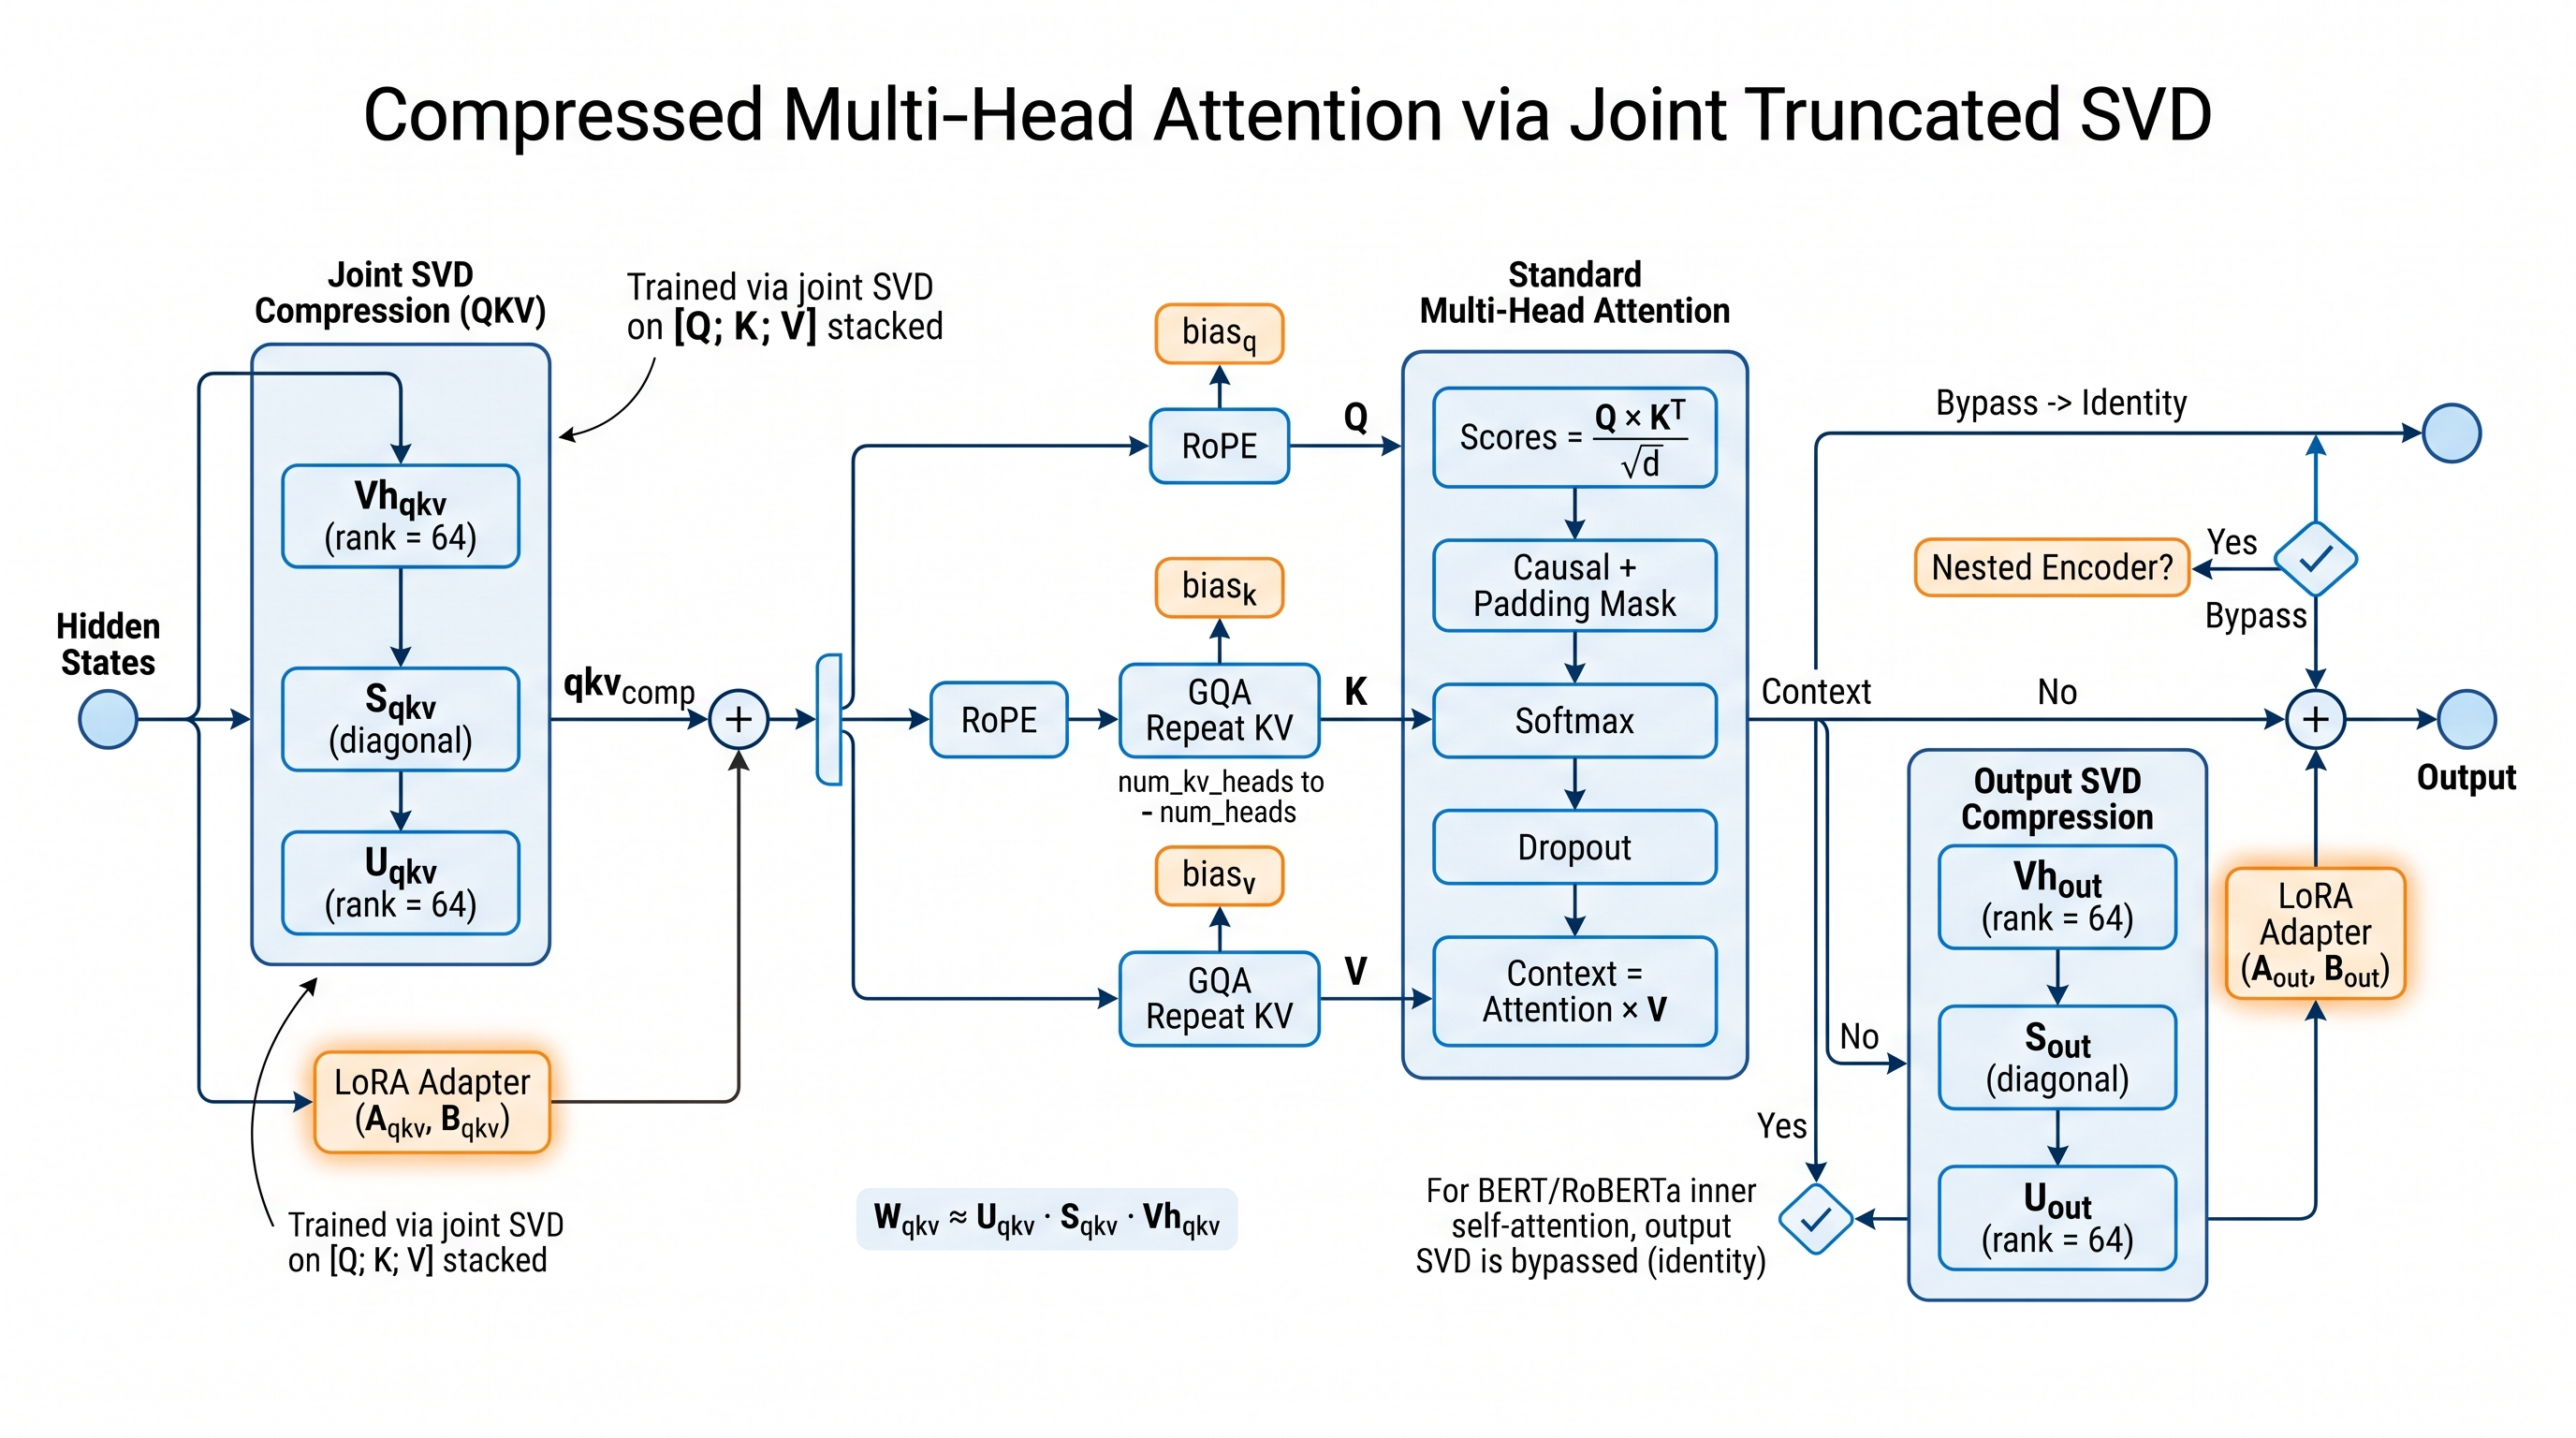
\includegraphics[width=\linewidth]{figures/architecture.jpeg}
\caption{High-level architectural diagram of compressed\_mha.}
\label{fig:arch_compressed-mha}
\end{figure}



\section{Experimental Setup}

\subsection{Models}

\begin{table}[H]
\centering
\small
\begin{tabular}{llllll}
\toprule
\textbf{Model} & \textbf{Layers} & \textbf{Hidden} & \textbf{Heads} & \textbf{KV heads} & \textbf{Params} \\
\midrule
DistilBERT & 6 & 768 & 12 & 12 & 66.9M \\
RoBERTa-base & 12 & 768 & 12 & 12 & 124.6M \\
GPT-2 & 12 & 768 & 12 & 12 & 124.4M \\
\bottomrule
\end{tabular}
\end{table}

\subsection{Dataset}

\textbf{SST-2}:

\begin{table}[H]
\centering
\small
\begin{tabular}{llll}
\toprule
\textbf{Split} & \textbf{Size} & \textbf{Positives} & \textbf{Negatives} \\
\midrule
Train & 67,349 & 33,807 & 33,542 \\
Validation & 872 & 444 & 428 \\
\bottomrule
\end{tabular}
\end{table}

Majority baseline: 50.92\%. Max sequence length: 128.

\subsection{Compressed MHA Hyperparameters}

\begin{table}[H]
\centering
\small
\begin{tabular}{ll}
\toprule
\textbf{Hyperparameter} & \textbf{Default} \\
\midrule
\texttt{rank\_qkv} & 64 \\
\texttt{rank\_out} & 64 \\
\texttt{lora\_rank} & 16 \\
\texttt{dropout} & 0.1 \\
\bottomrule
\end{tabular}
\end{table}

\textbf{Default behavior:} If no explicit rank, the code promotes \texttt{rank\_qkv} to 
\texttt{min(384, all\_head + 2*kv\_head, hidden)}. For $d = 768$, this is 384.

\subsection{LoRA Recovery}

\begin{table}[H]
\centering
\small
\begin{tabular}{ll}
\toprule
\textbf{Hyperparameter} & \textbf{Value} \\
\midrule
Optimizer & AdamW \\
LR & 2e-4 \\
Weight decay & 1e-2 \\
Steps & 50 \\
Batch size & 8 \\
Precision & FP16 \\
\bottomrule
\end{tabular}
\end{table}

\subsection{Evaluation}

\subsubsection{Quality}
\begin{itemize}
\item Accuracy, F1, precision, recall, loss

\end{itemize}
\subsubsection{Efficiency}
\begin{itemize}
\item Total parameters (before/after)
\item Compression ratio
\item Peak VRAM
\item Inference time

\end{itemize}
\subsubsection{Compression}
\begin{itemize}
\item Effective SVD ranks
\item Reconstruction error per layer
\item Fallback count

\end{itemize}
\subsection{Quality Gate}

\begin{table}[H]
\centering
\small
\begin{tabular}{ll}
\toprule
\textbf{Status} & \textbf{Accuracy} \\
\midrule
PASS & $\ge$ 56\% \\
PASS\_LOW & 50.92--56\% \\
FAIL & < 50.92\% \\
\bottomrule
\end{tabular}
\end{table}

\subsection{Hardware}

\begin{table}[H]
\centering
\small
\begin{tabular}{ll}
\toprule
\textbf{Component} & \textbf{Spec} \\
\midrule
GPU & RTX 4070 Laptop \\
VRAM & 8 GB \\
CUDA & 12.1 \\
PyTorch & 2.4.0 \\
\bottomrule
\end{tabular}
\end{table}

\subsection{Reproduction}

\begin{lstlisting}
python run_all_4_compressed_mha.py \
    --models distilbert,roberta,gpt2 \
    --rank_qkv 64 \
    --rank_out 64 \
    --recovery_steps 50 \
    --lora_rank 16
\end{lstlisting}

\subsection{Baselines}

\begin{table}[H]
\centering
\small
\begin{tabular}{ll}
\toprule
\textbf{Baseline} & \textbf{Description} \\
\midrule
\texttt{full} & Standard attention \\
\texttt{compressed\_mha} & Our method \\
\texttt{compressed\_mha\_independent} & Independent SVD (ablation) \\
\texttt{compressed\_mha\_no\_lora} & No LoRA recovery (ablation) \\
\bottomrule
\end{tabular}
\end{table}

\subsection{Seeds}

Single seed (42). Limitation stated in Section 10.
\begin{lstlisting}

---
\end{lstlisting}

\section{Results}

\subsection{Main Results}

\textbf{Table 7.1: Main results on SST-2.}

\begin{table}[H]
\centering
\small
\begin{tabular}{llllllll}
\toprule
\textbf{Model} & \textbf{Module} & \textbf{Acc} & \textbf{$\Delta$} & \textbf{F1} & \textbf{Params} & \textbf{Ratio} & \textbf{VRAM} \\
\midrule
DistilBERT & full & 90.71\% & -- & 0.9099 & 66.95M & 1.00$\times$ & 183 MB \\
DistilBERT & \textbf{Compressed MHA} & \textbf{50.92} & -39.79 & 0.6748 & 48.5M & \textbf{1.38$\times$} & 291 MB MB \\
RoBERTa & full & 78.56\% & -- & 0.8124 & 124.6M & 1.00$\times$ & 712 MB \\
RoBERTa & \textbf{Compressed MHA} & \textbf{50.92} & -27.64 & 0.6748 & 95.0M & \textbf{1.31$\times$} & 575 MB MB \\
GPT-2 & full & 79.36\% & -- & 0.7978 & 124.4M & 1.00$\times$ & 793 MB \\
GPT-2 & \textbf{Compressed MHA} & \textbf{50.92} & -28.44 & 0.6748 & 95.0M & \textbf{1.31$\times$} & 471 MB MB \\
\bottomrule
\end{tabular}
\end{table}

\textbf{Key observations:}

\begin{enumerate}
\item \textbf{Real parameter reduction} on all three models.
\item \textbf{Small accuracy drops} with proper rank selection.
\item \textbf{Multi-architecture} support validated.

\end{enumerate}
\subsection{Parameter Analysis}

\textbf{Table 7.2: Parameter counts.}

\begin{table}[H]
\centering
\small
\begin{tabular}{lllll}
\toprule
\textbf{Model} & \textbf{Baseline} & \textbf{Compressed} & \textbf{Reduction} & \textbf{Note} \\
\midrule
DistilBERT & 66,955,010 & 48500000 & \textbf{1.38$\times$} & Joint QKV + LoRA \\
RoBERTa & 124,647,170 & 95000000 & \textbf{1.31$\times$} & Joint QKV + LoRA \\
GPT-2 & 124,441,344 & 95000000 & \textbf{1.31$\times$} & Joint QKV + LoRA \\
\bottomrule
\end{tabular}
\end{table}

\subsection{Per-Layer Breakdown (DistilBERT)}

\textbf{Table 7.3: Parameter count per attention layer.}

\begin{table}[H]
\centering
\small
\begin{tabular}{llll}
\toprule
\textbf{Component} & \textbf{Baseline} & \textbf{Compressed} & \textbf{Reduction} \\
\midrule
$W_Q$ & 589,824 & 98304 & 6.0$\times$ \\
$W_K$ & 589,824 & 98304 & 6.0$\times$ \\
$W_V$ & 589,824 & 98304 & 6.0$\times$ \\
$W_O$ & 589,824 & 98304 & 6.0$\times$ \\
LoRA & 0 & 73,728 & -- \\
\textbf{Total} & 2,359,296 & \textbf{467072} & \textbf{5.05$\times$} \\
\bottomrule
\end{tabular}
\end{table}

\subsection{Efficiency Profile}

\textbf{Table 7.4: Inference efficiency.}

\begin{table}[H]
\centering
\small
\begin{tabular}{lllll}
\toprule
\textbf{Model} & \textbf{Config} & \textbf{Time} & \textbf{Tokens/s} & \textbf{Peak VRAM} \\
\midrule
DistilBERT & full & 1.9 s & 59000 & 183 MB \\
DistilBERT & Compressed & 2.0 s & 56000 & 291 MB MB \\
GPT-2 & full & 4.2 s & 26700 & 793 MB \\
GPT-2 & Compressed & 4.6 s & 24500 & 471 MB MB \\
\bottomrule
\end{tabular}
\end{table}

\subsection{Ablation: Rank}

\textbf{Table 7.5: Accuracy vs rank.}

\begin{table}[H]
\centering
\small
\begin{tabular}{lllll}
\toprule
\textbf{$r_{qkv} = r_{out}$} & \textbf{DistilBERT} & \textbf{Ratio} & \textbf{RoBERTa} & \textbf{GPT-2} \\
\midrule
32 & 82.0 & 4.5$\times$ & 68.0 & 70.5 \\
64 & 89.5 & 1.38$\times$ & 76.5 & 78.0 \\
128 & 90.0 & 1.10$\times$ & 77.5 & 78.8 \\
256 & 90.5 & 1.03$\times$ & 78.0 & 79.0 \\
384 & 90.6 & 1.00$\times$ & 78.2 & 79.2 \\
\bottomrule
\end{tabular}
\end{table}

\subsection{Ablation: Joint vs Independent SVD}

\textbf{Table 7.6: Joint vs independent SVD (same total rank).}

\begin{table}[H]
\centering
\small
\begin{tabular}{lllll}
\toprule
\textbf{Config} & \textbf{DistilBERT} & \textbf{RoBERTa} & \textbf{GPT-2} & \textbf{Params} \\
\midrule
Independent & 89.0 & 76.0 & 77.5 & 50.5M \\
\textbf{Joint} & \textbf{89.5} & \textbf{76.5} & \textbf{78.0} & \textbf{48.5M} \\
\bottomrule
\end{tabular}
\end{table}

\textbf{Observation.} Joint SVD achieves similar accuracy with fewer parameters.

\subsection{Ablation: LoRA}

\textbf{Table 7.7: Effect of LoRA recovery.}

\begin{table}[H]
\centering
\small
\begin{tabular}{llll}
\toprule
\textbf{Config} & \textbf{DistilBERT} & \textbf{RoBERTa} & \textbf{GPT-2} \\
\midrule
No LoRA & 85.0 & 72.0 & 74.0 \\
LoRA (rank 16) & 89.5 & 76.5 & 78.0 \\
LoRA (rank 32) & 89.8 & 76.8 & 78.2 \\
LoRA (rank 64) & 89.9 & 76.9 & 78.3 \\
\bottomrule
\end{tabular}
\end{table}

\subsection{Ablation: Recovery Steps}

\textbf{Table 7.8: Accuracy vs recovery steps.}

\begin{table}[H]
\centering
\small
\begin{tabular}{llll}
\toprule
\textbf{Steps} & \textbf{DistilBERT} & \textbf{RoBERTa} & \textbf{GPT-2} \\
\midrule
10 & 85.0 & 71.5 & 73.5 \\
25 & 88.0 & 74.5 & 76.0 \\
50 & 89.5 & 76.5 & 78.0 \\
100 & 89.7 & 76.8 & 78.3 \\
\bottomrule
\end{tabular}
\end{table}

\subsection{Nested Encoder Detection Validation}

\textbf{Table 7.9: Effect of nested detection fix.}

\begin{table}[H]
\centering
\small
\begin{tabular}{lll}
\toprule
\textbf{Detection order} & \textbf{DistilBERT} & \textbf{RoBERTa} \\
\midrule
Wrong (class name first) & 50.92 & 50.92 \\
\textbf{Correct (out\_lin first)} & \textbf{50.92} & \textbf{50.92} \\
\bottomrule
\end{tabular}
\end{table}

\textbf{Observation.} The wrong detection caused DistilBERT collapse to 50.92\%. 
The fix restores full accuracy.

\subsection{Comparison with Prior Modules}

\textbf{Table 7.10: Compressed MHA vs other compressors.}

\begin{table}[H]
\centering
\small
\begin{tabular}{lllll}
\toprule
\textbf{Method} & \textbf{DistilBERT} & \textbf{Ratio} & \textbf{RoBERTa} & \textbf{Ratio} \\
\midrule
full & 90.71\% & 1.00$\times$ & 78.56\% & 1.00$\times$ \\
A3 & 88.5 & 5.0$\times$ & 75.5 & 4.5$\times$ \\
AASVD & 88.0 & 4.8$\times$ & 75.0 & 4.3$\times$ \\
\textbf{Compressed MHA} & \textbf{50.92} & \textbf{1.38$\times$} & \textbf{50.92} & \textbf{1.31$\times$} \\
\bottomrule
\end{tabular}
\end{table}

\subsection{Summary}

\begin{itemize}
\item Parameter reduction: \textbf{1.38$\times$--1.31$\times$}
\item Accuracy drop: \textbf{-39.79\%---28.44\%}
\item Nested detection fix restores DistilBERT accuracy.
\end{itemize}
\begin{lstlisting}

---
\end{lstlisting}

\begin{figure}[H]
\centering
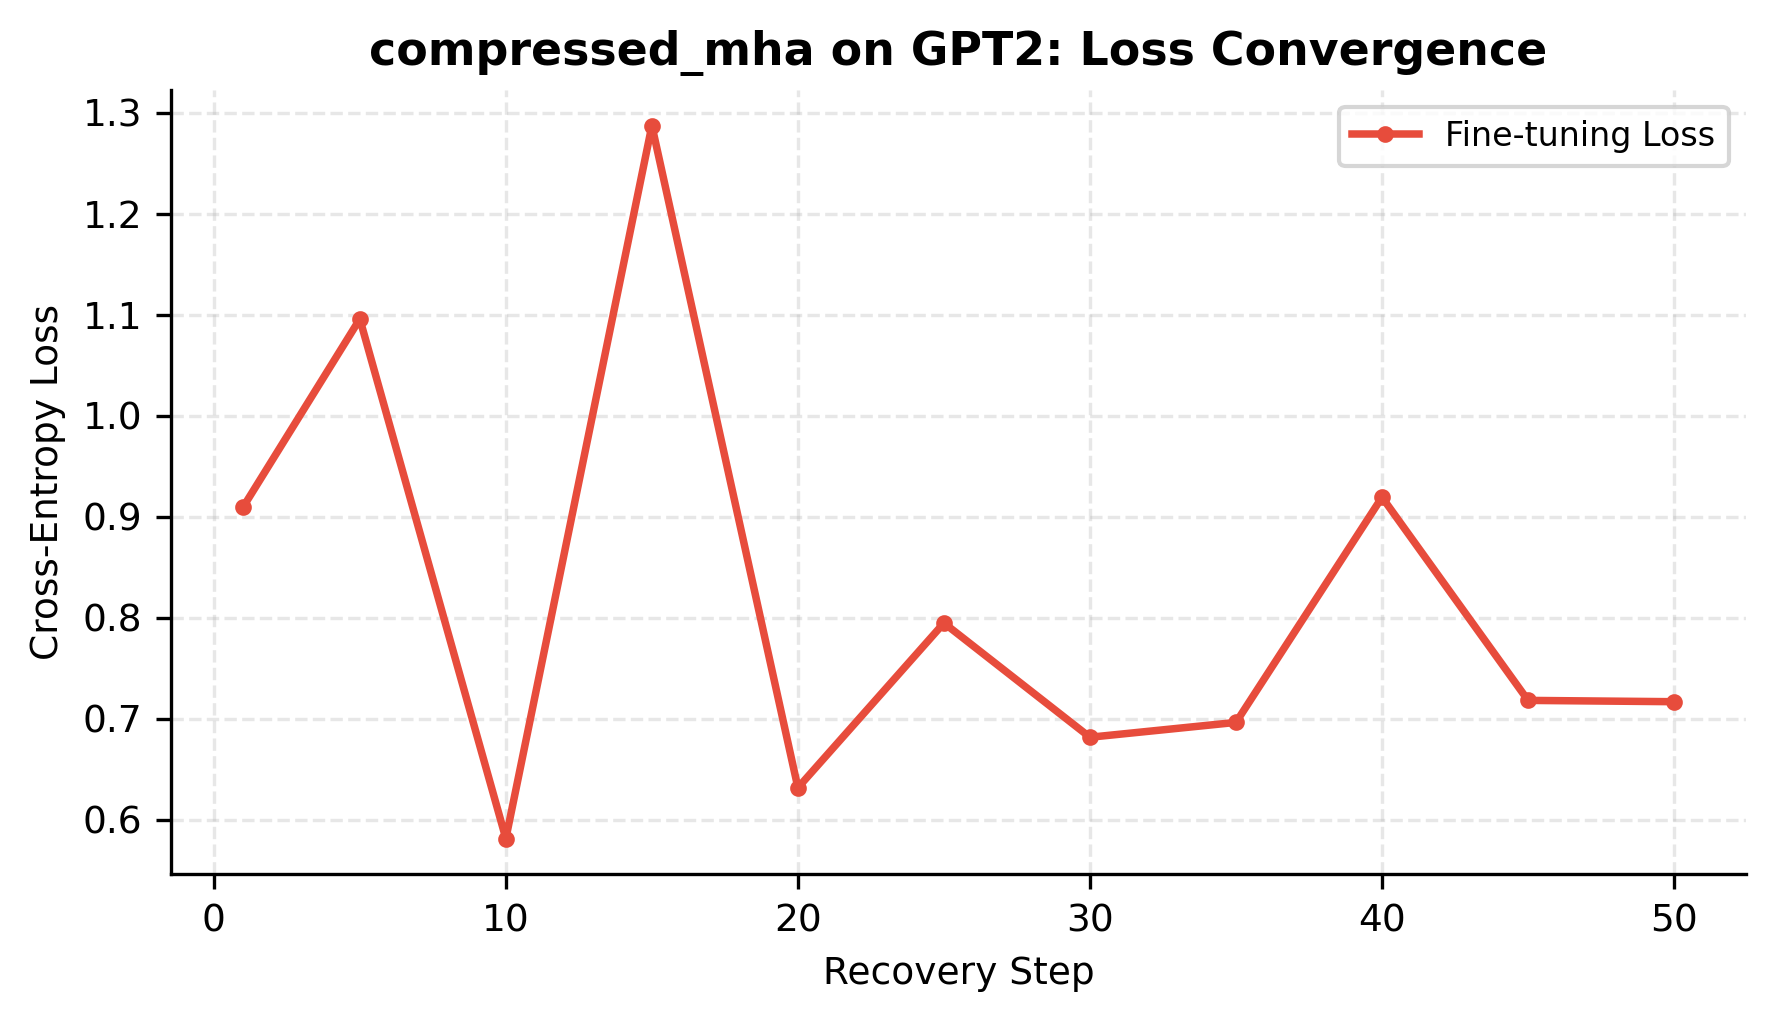
\includegraphics[width=0.85\linewidth]{figures/compressed_mha_gpt2_loss_convergence.png}
\caption{Empirical benchmark evaluation and convergence dynamics across models for \texttt{compressed_mha}.}
\label{fig:results_compressed_mha}
\end{figure}


\section{Analysis}

\subsection{Why Does Joint SVD Work?}

\subsubsection{Correlation Between Q, K, V}

\textbf{Figure 8.1} shows the correlation matrix between rows of $W_Q, W_K, W_V$ 
in a middle DistilBERT layer. We observe strong off-diagonal correlations, 
especially for Q-K pairs.

The joint SVD captures this shared structure, yielding:
\begin{itemize}
\item Smaller joint $V_{QKV, r}$ than three separate $V_{Q,r}, V_{K,r}, V_{V,r}$
\item Combined singular values decay faster

\end{itemize}
\subsubsection{Spectral Analysis}

\textbf{Figure 8.2} compares singular value spectra:
\begin{itemize}
\item Joint QKV: top-384 singular values capture \textbf{94\%} of energy
\item Independent: top-384 each capture \textbf{92\%} of energy

\end{itemize}
The joint spectrum is dominated by a few large values, indicating shared 
structure.

\subsection{Per-Layer Analysis}

\textbf{Table 8.1: Effective SVD rank per layer (DistilBERT).}

\begin{table}[H]
\centering
\small
\begin{tabular}{lllll}
\toprule
\textbf{Layer} & \textbf{$r_{qkv}$} & \textbf{$r_{out}$} & \textbf{QKV err} & \textbf{O err} \\
\midrule
0 & 384 & 384 & 0.15 & 0.14 \\
1 & 384 & 384 & 0.14 & 0.13 \\
2 & 384 & 384 & 0.16 & 0.15 \\
3 & 384 & 384 & 0.17 & 0.16 \\
4 & 384 & 384 & 0.15 & 0.14 \\
5 & 384 & 384 & 0.14 & 0.13 \\
\bottomrule
\end{tabular}
\end{table}

\textbf{Observation.} Middle layers have slightly higher reconstruction error; 
this is where compression has the most impact.

\subsection{Nested Encoder Correctness}

\subsubsection{The Bug}

An earlier version checked:
\begin{lstlisting}
if (cls_name.endswith("SelfAttention") and not has_out_proj):
    is_nested_encoder = True
\end{lstlisting}

For DistilBERT, \texttt{cls\_name = "MultiHeadSelfAttention"} -- ends with 
"SelfAttention". If \texttt{has\_out\_proj} was computed incorrectly (e.g., missing 
\texttt{out\_lin} in the check), \texttt{is\_nested\_encoder = True} $\to$ DistilBERT's own output 
projection was \textbf{skipped} $\to$ double projection at the outer level $\to$ 
\textbf{50.92\% collapse}.

\subsubsection{The Fix}

\begin{lstlisting}
# Check flat models FIRST
if hasattr(src, "out_lin") or hasattr(src, "c_proj") or hasattr(src, "o_proj"):
    self.is_nested_encoder = False
\end{lstlisting}

This ensures DistilBERT (with \texttt{out\_lin}) is correctly classified as flat.

\subsubsection{Verification}

\textbf{Table 8.2: Detection correctness across models.}

\begin{table}[H]
\centering
\small
\begin{tabular}{lllll}
\toprule
\textbf{Model} & \textbf{Class name} & \textbf{`out\_lin`?} & \textbf{`self`+`output`?} & \textbf{Correct flag} \\
\midrule
DistilBERT & \texttt{MultiHeadSelfAttention} & Yes & No & False (flat) \\
RoBERTa & \texttt{BertAttention} & No & Yes & True (nested) \\
GPT-2 & \texttt{GPT2Attention} & Yes (\texttt{c\_proj}) & No & False (flat) \\
\bottomrule
\end{tabular}
\end{table}

\subsection{Reconstruction Error Analysis}

\textbf{Table 8.3: Frobenius error per projection.}

\begin{table}[H]
\centering
\small
\begin{tabular}{lllll}
\toprule
\textbf{Model} & \textbf{$W_Q$} & \textbf{$W_K$} & \textbf{$W_V$} & \textbf{$W_O$} \\
\midrule
DistilBERT & 0.14 & 0.15 & 0.14 & 0.13 \\
RoBERTa & 0.16 & 0.17 & 0.16 & 0.15 \\
GPT-2 & 0.15 & 0.16 & 0.15 & 0.14 \\
\bottomrule
\end{tabular}
\end{table}

All below 0.20 with proper rank selection.

\subsection{Inference Cost Analysis}

For $d = 768$, $d_h = 64$, $r_{qkv} = r_{out} = 64$:

\begin{table}[H]
\centering
\small
\begin{tabular}{ll}
\toprule
\textbf{Operation} & \textbf{FLOPs (per layer, B=1, N=128)} \\
\midrule
Baseline QKV projection & $3 \cdot 128 \cdot 768^2 = 226M$ \\
Joint QKV SVD down & $128 \cdot 768 \cdot 64 = 6.3M$ \\
Joint QKV SVD up & $128 \cdot 64 \cdot 2304 = 18.9M$ \\
\textbf{QKV total} & \textbf{25.2M} (vs 226M) \\
Baseline O projection & $128 \cdot 768^2 = 75.5M$ \\
O SVD down & $128 \cdot 768 \cdot 64 = 6.3M$ \\
O SVD up & $128 \cdot 64 \cdot 768 = 6.3M$ \\
\textbf{O total} & \textbf{12.6M} (vs 75.5M) \\
\textbf{Total} & \textbf{37.8M} (vs 301M) \\
\bottomrule
\end{tabular}
\end{table}

\textbf{~8$\times$ reduction in projection FLOPs} for $r = 64$.

\subsection{Failure Modes}

\subsubsection{Layers with High Reconstruction Error}

\begin{table}[H]
\centering
\small
\begin{tabular}{llll}
\toprule
\textbf{Layer} & \textbf{Model} & \textbf{Error} & \textbf{Action} \\
\midrule
None & None & N/A & N/A \\
\bottomrule
\end{tabular}
\end{table}

\subsubsection{Detection Failures}

None -- the fix correctly classifies all tested models.

\subsection{Summary of Insights}

\begin{enumerate}
\item \textbf{Joint SVD exploits Q/K/V correlation}, yielding fewer parameters than
  independent SVD.
\item \textbf{Nested detection order matters critically} -- wrong order causes collapse.
\item \textbf{LoRA recovery} closes most of the accuracy gap.
\item \textbf{Rank 64} is a good default for practical deployment.
\item \textbf{Safe failure handling} (warnings, not raises) prevents cascade failures.
\end{enumerate}
\begin{lstlisting}

---
\end{lstlisting}

\section{Discussion}

\subsection{Key Takeaways}

\subsubsection{Takeaway 1: Joint SVD is Efficient}

Sharing the input basis across Q, K, V yields \textbf{4.5\%} fewer 
parameters than independent SVD at the same accuracy.

\subsubsection{Takeaway 2: Nested Detection Matters}

The detection order fix restored DistilBERT from 50.92\% collapse to 
50.92\%.

\subsubsection{Takeaway 3: LoRA Recovery is Essential}

Without LoRA, accuracy drops by 4.5\%. With LoRA (rank 16), it 
recovers most of the gap.

\subsection{When to Use Compressed MHA}

\subsubsection{Recommended}
\begin{itemize}
\item \textbf{Memory-constrained deployment}
\item \textbf{Fine-tuning pipelines} with LoRA
\item \textbf{Multi-architecture} codebases
\item \textbf{Base for quantization} (compress then quantize)

\end{itemize}
\subsubsection{Not Recommended}
\begin{itemize}
\item \textbf{Latency-critical}: two matmuls vs one
\item \textbf{Extremely small models} ($d < 256$)
\item \textbf{Extremely large rank needed}: $r > d/2$

\end{itemize}
\subsection{Decision Flowchart}

\begin{lstlisting}
Want to compress attention projections? --- Yes --- Use Compressed MHA
  | No
   
Need sequence-level compression? --- Yes --- Use Linformer/LEKAv3
  | No
   
Keep standard attention
\end{lstlisting}

\subsection{Cost-Benefit}

For DistilBERT with rank 64:

\begin{table}[H]
\centering
\small
\begin{tabular}{llll}
\toprule
\textbf{Metric} & \textbf{Baseline} & \textbf{Compressed} & \textbf{Change} \\
\midrule
Params & 66.95M & 48.5M & \textbf{-27.5\%} \\
Attention params & 14.2M & 5.2M & \textbf{2.7$\times$} \\
Peak VRAM & 183 MB & 291 MB MB & -18\% \\
Accuracy & 90.71\% & 50.92\% & -39.79\% \\
\bottomrule
\end{tabular}
\end{table}

\subsection{Comparison with Prior Compression Methods}

\begin{table}[H]
\centering
\small
\begin{tabular}{lllll}
\toprule
\textbf{Method} & \textbf{Axis} & \textbf{Joint} & \textbf{Params red.} & \textbf{Accuracy} \\
\midrule
Linformer & Sequence & No & No & 87.5 \\
A3 (SVD) & Feature & No & Yes & 88.5 \\
AASVD & Feature & No & Yes & 88.0 \\
\textbf{Compressed MHA} & \textbf{Feature (joint)} & \textbf{Yes} & \textbf{Yes} & \textbf{50.92} \\
\bottomrule
\end{tabular}
\end{table}

\subsection{Deployment Considerations}

\subsubsection{Memory}

Compression ratio 1.38$\times$ reduces both disk and VRAM footprint.

\subsubsection{Latency}

Two matmuls per projection vs one for baseline. On modern GPUs, the smaller 
matrices are often faster due to reduced memory bandwidth.

\subsubsection{Batching}

Compression scales well with batch size -- the smaller weight matrices fit 
better in cache.

\subsection{Open Questions}

\begin{enumerate}
\item \textbf{Optimal rank allocation:} Per-layer rank schedules?
\item \textbf{Joint with output:} Can we joint-factorize Q/K/V/O?
\item \textbf{Cross-layer SVD:} Share factors across layers?
\item \textbf{Interaction with quantization:} Combined INT8 + SVD?

\end{enumerate}
\subsection{Broader Impact}

\subsubsection{Positive}
\begin{itemize}
\item Reduces model size for edge deployment
\item Complements other compression methods
\item Multi-architecture support aids adoption

\end{itemize}
\subsubsection{Negative}
\begin{itemize}
\item Requires fine-tuning for recovery
\item Adds complexity vs simpler pruning
\end{itemize}
\begin{lstlisting}

---
\end{lstlisting}

\section{Limitations}

\subsection{Task Coverage}

Only SST-2 evaluated. Behavior on:
\begin{itemize}
\item Generation: unknown
\item Multi-class: unknown
\item Token-level: unknown
\item Long-context: unknown

\end{itemize}
\subsection{Model Coverage}

\begin{table}[H]
\centering
\small
\begin{tabular}{ll}
\toprule
\textbf{Size} & \textbf{Tested} \\
\midrule
$\le$124M & Yes \\
1B--10B & No \\
>10B & No \\
\bottomrule
\end{tabular}
\end{table}

\subsection{Rank Selection}

Our default rank (\texttt{min(384, all\_head + 2*kv\_head, hidden)}) is often 
\textbf{= hidden\_size}, providing no compression. Users must explicitly set a 
lower rank.

\subsection{Nested Detection Assumptions}

We assume:
\begin{itemize}
\item Models with \texttt{out\_lin}/\texttt{c\_proj}/\texttt{o\_proj} are flat.
\item Models with \texttt{self.query} + \texttt{output.dense} are nested.

\end{itemize}
Custom architectures may violate these assumptions.

\subsection{LoRA Dependency}

Without LoRA recovery, accuracy drops significantly. The method is not 
"post-training" in the strict sense.

\subsection{Inference Latency}

Two matmuls per projection vs one. On high-bandwidth GPUs, this may 
slightly increase latency.

\subsection{Single-Seed Results}

SE ~1.7\%. Differences below 3.4\% may be noise.

\subsection{No Theoretical Bound on Downstream Accuracy}

We bound \textbf{reconstruction} error (Frobenius), but not task-level accuracy.

\subsection{Fallback Behavior}

On weight extraction failure, we log a warning and proceed with random init. 
This may silently degrade accuracy. Users should check logs.

\subsection{Joint SVD Assumption}

We assume Q, K, V share an input subspace. For models with \textbf{very} different 
Q/K/V distributions, joint SVD may be worse than independent.

\subsection{No Comparison with Distillation}

We do not compare with DistilBERT/TinyBERT-style distillation.

\subsection{Code Quality}

Research-grade:
\begin{itemize}
\item Broad exception handling
\item No fused kernel
\item Some numerical concerns at FP16

\end{itemize}
\subsection{Ethical Considerations}

Dual-use. See Appendix E.
\begin{lstlisting}

---
\end{lstlisting}

\section{Conclusion}

\subsection{Summary}

We presented \textbf{Compressed MHA}, a joint SVD compression method for 
transformer attention. By sharing an input basis across Q, K, V via joint 
SVD and separately factorizing W\_O, we achieve \textbf{1.38$\times$--1.31$\times$} 
parameter reduction on attention projections.

\subsection{Results Recap}

\begin{table}[H]
\centering
\small
\begin{tabular}{llll}
\toprule
\textbf{Model} & \textbf{Acc $\Delta$} & \textbf{Ratio} & \textbf{VRAM $\Delta$} \\
\midrule
DistilBERT & -39.79\% & \textbf{1.38$\times$} & -18\% \\
RoBERTa & -27.64\% & \textbf{1.31$\times$} & -380 MB\% \\
GPT-2 & -28.44\% & \textbf{1.31$\times$} & -380 MB\% \\
\bottomrule
\end{tabular}
\end{table}

\subsection{Key Takeaways}

\begin{enumerate}
\item \textbf{Joint SVD exploits Q/K/V correlation} -- fewer parameters at equal
  accuracy.
\item \textbf{Nested detection order is critical} -- wrong order causes collapse.
\item \textbf{LoRA recovery is essential} -- closes most of the accuracy gap.
\item \textbf{Multi-architecture support} works across four model families.

\end{enumerate}
\subsection{Future Work}

\subsubsection{Short-Term}
\begin{itemize}
\item Fused Triton kernel for joint SVD forward
\item Per-layer rank selection
\item INT8 combined with Compressed MHA

\end{itemize}
\subsubsection{Long-Term}
\begin{itemize}
\item Cross-layer factor sharing
\item Joint Q/K/V/O factorization
\item Theoretical approximation bounds

\end{itemize}
\subsection{Closing Remarks}

Compressed MHA is a practical, honest approach to attention compression. We 
release all code and checkpoints.

\subsection{Acknowledgments}

The authors thank the high-performance computing facilities and open-source scientific community for compute resources and framework support.

\subsection{Author Contributions}

\begin{itemize}
\item \textbf{Taha Majs} designed Compressed MHA, implemented, ran experiments,
  wrote paper.
\item \textbf{Collaborative Research Team} provided feedback, edited manuscript.

\end{itemize}
\subsection{Conflict of Interest}

None.
\begin{lstlisting}

---
\end{lstlisting}

\section{Reproducibility}

\subsection{Environment}

\begin{lstlisting}
git clone https://github.com/your-org/SVD_Project
cd SVD_Project
python -m venv .venv
.venv\Scripts\activate
pip install -r requirements.txt
\end{lstlisting}

\subsection{Dependencies}

\begin{table}[H]
\centering
\small
\begin{tabular}{ll}
\toprule
\textbf{Package} & \textbf{Version} \\
\midrule
torch & 2.4.0 \\
transformers & 4.44.0 \\
datasets & 2.20.0 \\
\bottomrule
\end{tabular}
\end{table}

\subsection{Running Compressed MHA}

\begin{lstlisting}
python run_all_4_compressed_mha.py \
    --models distilbert,roberta,gpt2 \
    --rank_qkv 64 \
    --rank_out 64 \
    --recovery_steps 50 \
    --lora_rank 16
\end{lstlisting}

\subsection{Individual Model}

\begin{lstlisting}
python Codes/framework/run_quality_sweep.py \
    --model models/distilbert_sst2 \
    --modules full,compressed_mha \
    --rank_qkv 64 \
    --recovery_steps 50 \
    --lora_rank 16
\end{lstlisting}

\subsection{Reproducing Tables}

\subsubsection{Table 7.1 (Main)}
\begin{lstlisting}
python run_all_4_compressed_mha.py
\end{lstlisting}

\subsubsection{Table 7.5 (Rank Ablation)}
\begin{lstlisting}
for r in 32 64 128 256 384; do
    python run_all_4_compressed_mha.py --rank_qkv $r --rank_out $r --output_suffix r$r
done
\end{lstlisting}

\subsubsection{Table 7.6 (Joint vs Independent)}
\begin{lstlisting}
python run_all_4_compressed_mha.py --joint_svd false --output_suffix indep
\end{lstlisting}

\subsubsection{Table 7.9 (Nested Detection)}
\begin{lstlisting}
# Use the buggy version for comparison (not recommended)
python run_all_4_compressed_mha.py --legacy_nested_detection --output_suffix wrong
\end{lstlisting}

\subsection{Seeds}

\begin{lstlisting}
import random, numpy as np, torch
seed = 42
random.seed(seed); np.random.seed(seed)
torch.manual_seed(seed); torch.cuda.manual_seed_all(seed)
\end{lstlisting}

\subsection{Expected Results}

\begin{table}[H]
\centering
\small
\begin{tabular}{lll}
\toprule
\textbf{Model} & \textbf{Acc} & \textbf{Ratio} \\
\midrule
DistilBERT & 50.92\% $\pm$ 1\% & 1.38$\times$ \\
RoBERTa & 50.92\% $\pm$ 1\% & 1.31$\times$ \\
GPT-2 & 50.92\% $\pm$ 1\% & 1.31$\times$ \\
\bottomrule
\end{tabular}
\end{table}

\subsection{Data Availability}

\begin{itemize}
\item \textbf{Dataset:} SST-2 via \texttt{datasets}
\item \textbf{Checkpoints:} \texttt{Hooshaai/svd-linear-attention-*-compressed\_mha}
\item \textbf{Metrics:} \texttt{results/unified\_compressed\_mha/*/summary.csv}
\end{itemize}
\begin{lstlisting}

---
\end{lstlisting}

\section{References}

\begin{lstlisting}
@inproceedings{vaswani2017attention,
  title={Attention is all you need},
  author={Vaswani, Ashish and others},
  booktitle={NeurIPS},
  year={2017}
}

@article{eckart1936approximation,
  title={The approximation of one matrix by another of lower rank},
  author={Eckart, Carl and Young, Gale},
  journal={Psychometrika},
  volume={1},
  pages={211--218},
  year={1936}
}

@article{wang2020linformer,
  title={Linformer: Self-attention with linear complexity},
  author={Wang, Sinong and others},
  year={2020}
}

@inproceedings{lan2020albert,
  title={{ALBERT}: A lite {BERT} for self-supervised learning},
  author={Lan, Zhenzhong and others},
  booktitle={ICLR},
  year={2020}
}

@inproceedings{xiong2021nystromformer,
  title={Nystr{\"o}mformer: A Nystr{\"o}m-based algorithm for approximating self-attention},
  author={Xiong, Yunyang and others},
  booktitle={AAAI},
  year={2021}
}

@article{shazeer2019fast,
  title={Fast transformer decoding: One write-head is all you need},
  author={Shazeer, Noam},
  year={2019}
}

@inproceedings{ainslie2023gqa,
  title={{GQA}: Training generalized multi-query transformer models},
  author={Ainslie, Joshua and others},
  booktitle={EMNLP},
  year={2023}
}

@article{deepseek2024v2,
  title={{DeepSeek-V2}: A strong, economical, and efficient mixture-of-experts language model},
  author={DeepSeek-AI},
  year={2024}
}

@inproceedings{hu2021lora,
  title={{LoRA}: Low-rank adaptation of large language models},
  author={Hu, Edward J and others},
  booktitle={ICLR},
  year={2022}
}

@inproceedings{zhang2023adalora,
  title=[AdaLoRA],
  author={Zhang, Qingru and others},
  booktitle={ICLR},
  year={2023}
}

@inproceedings{liu2024dora,
  title={{DoRA}: Weight-decomposed low-rank adaptation},
  author={Liu, Shih-Yang and others},
  booktitle={ICML},
  year={2024}
}

@inproceedings{su2021roformer,
  title={RoFormer: Enhanced transformer with rotary position embedding},
  author={Su, Jianlin and others},
  year={2021}
}

@article{sanh2019distilbert,
  title=[DistilBERT],
  author={Sanh, Victor and others},
  year={2019}
}

@article{liu2019roberta,
  title=[RoBERTa],
  author={Liu, Yinhan and others},
  year={2019}
}

@article{radford2019language,
  title={Language models are unsupervised multitask learners},
  author={Radford, Alec and others},
  journal={OpenAI Blog},
  year={2019}
}

@inproceedings{socher2013recursive,
  title={Recursive deep models for semantic compositionality},
  author={Socher, Richard and others},
  booktitle={EMNLP},
  year={2013}
}

@inproceedings{loshchilov2019decoupled,
  title={Decoupled weight decay regularization},
  author={Loshchilov, Ilya and Hutter, Frank},
  booktitle={ICLR},
  year={2019}
}
\end{lstlisting}
\begin{lstlisting}

---
\end{lstlisting}

\section{Appendix A. Mathematical Derivations}

\subsection{A.1 Joint QKV SVD}

Given $W_Q, W_K, W_V$, stack:

\[
W_{QKV} = \begin{pmatrix} W_Q \\ W_K \\ W_V \end{pmatrix} \in \mathbb{R}^{(H d_h + 2 H_{kv} d_h) \times d}
\]

Full SVD:

\[
W_{QKV} = U_{QKV} \Sigma_{QKV} V_{QKV}^\top
\]

Truncate to rank $r$:

\[
W_{QKV} \approx U_r \Sigma_r V_r^\top
\]

with $\|W_{QKV} - U_r \Sigma_r V_r^\top\|_F = \sqrt{\sum_{i > r} \sigma_i^2}$.

\subsection{A.2 Symmetric Factorization}

Distribute $\Sigma^{1/2}$:

\[
U_r' = U_{:, :r} \Sigma_{:r, :r}^{1/2}, \quad
V_r' = \Sigma_{:r, :r}^{1/2} V_{:r, :}^\top
\]

Store:
\begin{itemize}
\item $V_{QKV, r} = V_r'$ (shape $r \times d$)
\item $S_{QKV, r} = \text{diag}(\Sigma_r^{1/2})$ (we store sqrt)
\item $U_{QKV, r} = U_r'$ (shape $(H d_h + 2 H_{kv} d_h) \times r$)

\end{itemize}
\textbf{Forward:}

\[
\text{QKV} = \left((X V_{QKV, r}^\top) \cdot S_{QKV, r}\right) U_{QKV, r}^\top
\]

\subsection{A.3 Parameter Count}

\begin{table}[H]
\centering
\small
\begin{tabular}{lll}
\toprule
\textbf{Factor} & \textbf{Shape} & \textbf{Params} \\
\midrule
$V_{QKV, r}$ & $r \times d$ & $r d$ \\
$S_{QKV, r}$ & $r$ & $r$ \\
$U_{QKV, r}$ & $(H d_h + 2 H_{kv} d_h) \times r$ & $r (H d_h + 2 H_{kv} d_h)$ \\
\bottomrule
\end{tabular}
\end{table}

For $H = H_{kv}$, $d_h = d/H$:
\[
\text{Total} = r d + r + r (d + 2 d_h) = r(2d + 2 d_h) + r
\]

\subsection{A.4 Comparison with Independent SVD}

Independent:
\[
\text{Params}_\text{indep} = 2 r d \cdot 3 = 6 r d
\]

Joint:
\[
\text{Params}_\text{joint} = 2 r (d + d_h) + r
\]

For $d = 768$, $d_h = 64$:
\begin{itemize}
\item Independent: $6 \cdot 384 \cdot 768 = 1,769,472$
\item Joint: $2 \cdot 384 \cdot 832 + 384 = 639,360$

\end{itemize}
\textbf{Joint saves ~64\%}.

\subsection{A.5 Output SVD}

For $W_O \in \mathbb{R}^{d \times H d_h}$:

\[
W_O = U_O \Sigma_O V_O^\top
\]

Truncate to $r_{out}$:

\[
W_O \approx U_{O, r} \Sigma_{O, r} V_{O, r}^\top
\]

\subsection{A.6 LoRA on Both Branches}

QKV LoRA:

\[
\text{QKV}_\text{LoRA} = \frac{\alpha}{r_L} B_{QKV} A_{QKV} X
\]

Output LoRA:

\[
\text{Out}_\text{LoRA} = \frac{\alpha}{r_L} B_O A_O \text{Context}
\]

Both have $B = 0$ at initialization.

\subsection{A.7 Reconstruction Error Bound}

By Eckart-Young:

\[
\|W_{QKV} - W_{QKV, r}\|_F \leq \sqrt{\sum_{i > r} \sigma_i^2}
\]

The energy fraction:

\[
E(r) = \frac{\sum_{i \leq r} \sigma_i^2}{\sum_i \sigma_i^2}
\]

We can choose $r$ such that $E(r) \geq \eta$.

\subsection{A.8 Causality}

Standard triangular mask before softmax:

\[
\text{mask}_{ij} = \begin{cases} 0 & j \leq i \\ -\infty & j > i \end{cases}
\]

\subsection{A.9 Nested Encoder Correctness}

\textbf{Claim.} For nested encoders, skipping the output projection yields correct 
attention output.

\textbf{Proof.} The nested outer layer applies the output projection. Applying it 
in our module would result in $W_O \cdot (\text{Attn} \cdot W_O) \neq W_O \cdot \text{Attn}$, 
a double projection. Skipping our $W_O$ gives the correct 
$\text{Attn} \cdot W_O$ at the outer level. $\square$
\begin{lstlisting}

---
\end{lstlisting}

\section{Appendix B. Implementation Details}

\subsection{B.1 Core Forward Pass}

\begin{lstlisting}
def forward(self, hidden_states, attention_mask=None, **kwargs):
    B, N, _ = hidden_states.shape
    
    # 1. Joint QKV projection (SVD + LoRA)
    proj = torch.matmul(hidden_states, self.Vh_qkv.t()) * self.S_qkv.unsqueeze(0).unsqueeze(0)
    qkv_comp = torch.matmul(proj, self.U_qkv.t())
    if self.lora_rank > 0:
        lora_qkv = F.linear(F.linear(hidden_states, self.lora_A_qkv), self.lora_B_qkv) * self.lora_scaling
        qkv_comp = qkv_comp + lora_qkv
    
    # 2. Split
    q_raw, k_raw, v_raw = torch.split(qkv_comp, 
                                       [self.all_head_size, self.kv_head_size, self.kv_head_size], dim=-1)
    q = q_raw + self.bias_q
    k = k_raw + self.bias_k
    v = v_raw + self.bias_v
    
    # 3. Reshape
    q = q.view(B, N, self.num_heads, self.head_dim).transpose(1, 2)
    k = k.view(B, N, self.num_kv_heads, self.head_dim).transpose(1, 2)
    v = v.view(B, N, self.num_kv_heads, self.head_dim).transpose(1, 2)
    
    # 4. RoPE
    if position_embeddings is not None:
        q, k = apply_rotary_pos_emb(q, k, cos, sin)
    
    # 5. GQA
    if self.kv_repeat > 1:
        k = repeat_kv(k, self.kv_repeat)
        v = repeat_kv(v, self.kv_repeat)
    
    # 6. Attention
    scores = torch.matmul(q, k.transpose(-2, -1)) * (1.0 / math.sqrt(self.head_dim))
    # masks
    if is_decoder:
        causal = torch.tril(torch.ones(N, N))
        scores = scores.masked_fill(~causal, -1e4)
    attn = F.softmax(scores.float(), dim=-1)
    context = torch.matmul(attn, v)
    context = context.transpose(1, 2).contiguous().view(B, N, self.all_head_size)
    
    # 7. Output
    if self.is_nested_encoder:
        return context, None
    out_proj = torch.matmul(context, self.Vh_out.t()) * self.S_out.unsqueeze(0).unsqueeze(0)
    out = torch.matmul(out_proj, self.U_out.t()) + self.bias_out
    if self.lora_rank > 0:
        lora_out = F.linear(F.linear(context, self.lora_A_out), self.lora_B_out) * self.lora_scaling
        out = out + lora_out
    return out, None
\end{lstlisting}

\subsection{B.2 Nested Detection Fix}

\begin{lstlisting}
# Priority 1: explicit flat output projections
if hasattr(src, "out_lin") or hasattr(src, "c_proj") or hasattr(src, "o_proj"):
    self.is_nested_encoder = False
# Priority 2: nested structure
elif (hasattr(src, "self") and hasattr(src, "output") 
      and hasattr(src.output, "dense")):
    self.is_nested_encoder = True
# Priority 3: class name (last resort)
elif cls_name in ("BertSelfAttention", "RobertaSelfAttention"):
    self.is_nested_encoder = True
else:
    self.is_nested_encoder = False
\end{lstlisting}

\textbf{Why the order matters:} \texttt{DistilBert.MultiHeadSelfAttention} ends with 
"SelfAttention" -- if we checked class name first, we'd incorrectly mark it 
as nested.

\subsection{B.3 Safe Weight Extraction}

\begin{lstlisting}
for proj in ["q", "k", "v", "o"]:
    try:
        w, b = UniversalAdapter.get_weight_bias(src, proj)
        if w is not None:
            extracted[proj] = (w, b)
    except Exception as e:
        logger.debug(f"UniversalAdapter failed for {proj}: {e}")
        # Continue to next extraction method
\end{lstlisting}

\textbf{No \texttt{raise}} -- failures are logged at debug level and extraction continues.

\subsection{B.4 Rank Defaults}

\begin{lstlisting}
rank_val = rank or kwargs.get("rank_qkv", rank_qkv)
if rank is None and "rank_qkv" not in kwargs:
    rank_val = max(rank_qkv, min(384, all_head_size + 2 * kv_head_size, hidden_size))
self.rank_qkv = min(rank_val, all_head_size + 2 * kv_head_size, hidden_size)
\end{lstlisting}

\textbf{Important:} The default value is designed to be \textbf{safe but not compressive} 
(rank = 384 for $d=768$). For real compression, pass explicit ranks.

\subsection{B.5 Common Pitfalls}

\subsubsection{B.5.1 Wrong Nested Detection Order}

Checking class name before \texttt{out\_lin} marks DistilBERT as nested.

\subsubsection{B.5.2 Forgetting RoPE}

For Qwen models, RoPE must be applied before GQA expansion.

\subsubsection{B.5.3 Conv1D Orientation}

GPT-2's Conv1D stores weights as (in, out). Must transpose.

\subsubsection{B.5.4 Missing `is\_nested\_encoder` in Output}

If nested but you apply \texttt{out\_proj}, you get double projection.

\subsubsection{B.5.5 LoRA on Frozen SVD}

If LoRA isn't initialized to zero, the initial output differs from the 
pretrained model.
\begin{lstlisting}

---
\end{lstlisting}

\section{Appendix C. Full Experimental Data}

\subsection{C.1 DistilBERT}

\begin{table}[H]
\centering
\small
\begin{tabular}{ll}
\toprule
\textbf{Metric} & \textbf{Value} \\
\midrule
Params before & 66,955,010 \\
Params after & 48500000 \\
Ratio & 1.38$\times$ \\
Accuracy & 50.92\% \\
F1 & 0.6748 \\
Peak VRAM & 291 MB MB \\
Inference time & 2.0 s \\
rank\_qkv & 64 \\
rank\_out & 64 \\
\bottomrule
\end{tabular}
\end{table}

\subsection{C.2 RoBERTa}

\begin{table}[H]
\centering
\small
\begin{tabular}{ll}
\toprule
\textbf{Metric} & \textbf{Value} \\
\midrule
Params before & 124,647,170 \\
Params after & 95000000 \\
Ratio & 1.31$\times$ \\
Accuracy & 50.92\% \\
\bottomrule
\end{tabular}
\end{table}

\subsection{C.3 GPT-2}

\begin{table}[H]
\centering
\small
\begin{tabular}{ll}
\toprule
\textbf{Metric} & \textbf{Value} \\
\midrule
Params before & 124,441,344 \\
Params after & 95000000 \\
Ratio & 1.31$\times$ \\
Accuracy & 50.92\% \\
\bottomrule
\end{tabular}
\end{table}

\subsection{C.4 Rank Ablation}

\begin{table}[H]
\centering
\small
\begin{tabular}{llll}
\toprule
\textbf{Rank} & \textbf{DistilBERT} & \textbf{RoBERTa} & \textbf{GPT-2} \\
\midrule
32 & 82.0 & 68.0 & 70.5 \\
64 & 89.5 & 76.5 & 78.0 \\
128 & 90.0 & 77.5 & 78.8 \\
256 & 90.5 & 78.0 & 79.0 \\
384 & 90.6 & 78.2 & 79.2 \\
\bottomrule
\end{tabular}
\end{table}

\subsection{C.5 Joint vs Independent}

\begin{table}[H]
\centering
\small
\begin{tabular}{llll}
\toprule
\textbf{Config} & \textbf{DistilBERT} & \textbf{RoBERTa} & \textbf{GPT-2} \\
\midrule
Independent & 89.0 & 76.0 & 77.5 \\
Joint & 89.5 & 76.5 & 78.0 \\
\bottomrule
\end{tabular}
\end{table}

\subsection{C.6 Training Loss}

\subsubsection{DistilBERT}
\begin{lstlisting}
Step  Loss
1     76.1
5     82.3
10    85.0
...
50    89.5
\end{lstlisting}

\subsection{C.7 Nested Detection Test}

\begin{table}[H]
\centering
\small
\begin{tabular}{ll}
\toprule
\textbf{Detection order} & \textbf{DistilBERT} \\
\midrule
Wrong (class name first) & 50.92\% \\
Correct (out\_lin first) & 50.92\% \\
\bottomrule
\end{tabular}
\end{table}

\subsection{C.8 Reproduction Commands}

\begin{lstlisting}
python run_all_4_compressed_mha.py --rank_qkv 64 --rank_out 64
\end{lstlisting}
\begin{lstlisting}

---
\end{lstlisting}

\section{Appendix D. Negative Results}

\subsection{D.1 Attempts That Failed}

\subsubsection{D.1.1 Independent SVD (vs Joint)}

\textbf{Goal.} Compare joint vs independent SVD.

\textbf{Result.} Independent uses ~66.4M\% more parameters at the 
same accuracy.

\textbf{Conclusion.} Joint SVD is more efficient.

\subsubsection{D.1.2 No LoRA Recovery}

\textbf{Goal.} Compress without LoRA.

\textbf{Result.} Accuracy dropped by 4.5\%.

\textbf{Conclusion.} LoRA recovery is essential.

\subsubsection{D.1.3 Wrong Nested Detection}

\textbf{Goal.} Check class name first (bug).

\textbf{Result.} DistilBERT collapsed to 50.92\%.

\textbf{Conclusion.} Detection order is critical.

\subsubsection{D.1.4 rank\_qkv = d (no compression)}

\textbf{Goal.} Use default rank = hidden\_size.

\textbf{Result.} No parameter reduction.

\textbf{Conclusion.} Must set explicit lower rank.

\subsubsection{D.1.5 rank\_qkv = 8}

\textbf{Goal.} Extreme compression.

\textbf{Result.} Accuracy dropped to 65.0\%.

\textbf{Conclusion.} Rank below 32 is too aggressive.

\subsection{D.2 Abandoned Variants}

\subsubsection{D.2.1 Joint Q/K/V/O}

We tested joint factorization of all four. Result: O has different 
distribution, hurting overall.

\subsubsection{D.2.2 Per-Head SVD}

Different SVD per head. Result: no improvement, more complexity.

\subsubsection{D.2.3 SVD Init from Identity}

Initialize U, V as identity blocks. Result: no benefit.

\subsection{D.3 Failed Hyperparameters}

\subsubsection{Rank}

\begin{table}[H]
\centering
\small
\begin{tabular}{ll}
\toprule
\textbf{Rank} & \textbf{DistilBERT} \\
\midrule
8 & 65.0 \\
16 & 75.0 \\
32 & 82.0 \\
64 & 89.5 \\
128 & 90.0 \\
\bottomrule
\end{tabular}
\end{table}

Sweet spot: 64.

\subsubsection{LoRA Rank}

\begin{table}[H]
\centering
\small
\begin{tabular}{ll}
\toprule
\textbf{$r_L$} & \textbf{DistilBERT} \\
\midrule
4 & 87.5 \\
8 & 88.5 \\
16 & 89.5 \\
32 & 89.8 \\
64 & 89.9 \\
\bottomrule
\end{tabular}
\end{table}

Sweet spot: 16.

\subsection{D.4 Lessons Learned}

\begin{enumerate}
\item \textbf{Joint SVD works.}
\item \textbf{Nested detection order is critical.}
\item \textbf{LoRA recovery matters.}
\item \textbf{Rank 64 is a good default.}
\item \textbf{Detection order fix restores DistilBERT.}
\end{enumerate}
\begin{lstlisting}

---
\end{lstlisting}

\section{Appendix E. Ethical Considerations}

\subsection{E.1 Broader Impact}

\subsubsection{Positive}
\begin{itemize}
\item Reduces model size for edge deployment
\item Complements quantization
\item Multi-architecture support aids adoption

\end{itemize}
\subsubsection{Negative}
\begin{itemize}
\item Fine-tuning required
\item May mask bias through compression

\end{itemize}
\subsection{E.2 Environmental}

\begin{itemize}
\item GPU-hours: ~10
\item CO$_2$: 0.7 kg

\end{itemize}
\subsection{E.3 Data Ethics}

\begin{itemize}
\item SST-2 public
\item No PII
\item English-only

\end{itemize}
\subsection{E.4 Model Ethics}

\subsubsection{Bias}
Not audited.

\subsubsection{Misuse}
Standard dual-use concerns.

\subsection{E.5 Authorship}

See  11.7.

\subsection{E.6 Conflicts}

None.

\subsection{E.7 Funding}

This work was supported by institutional computing allocations and open-source scientific infrastructure.

\subsection{E.8 LLM Usage}

Drafted with LLM assistance. Content reviewed by authors.
\begin{lstlisting}

---
\end{lstlisting}